\section{Spatial distributions of correlations}
Considering the correlations between the different variables, we can look at the spatial distribution of Antarctic SIE with the different indices. Starting with the raw data from each grid point correlated with the different indices we get the following figure. We note that most of the correlations here are weak and insignificant. This is probably due to the seasonal cycle being the dominating factor in the time series before anything else is done.
\begin{figure}[H]
    \centering
    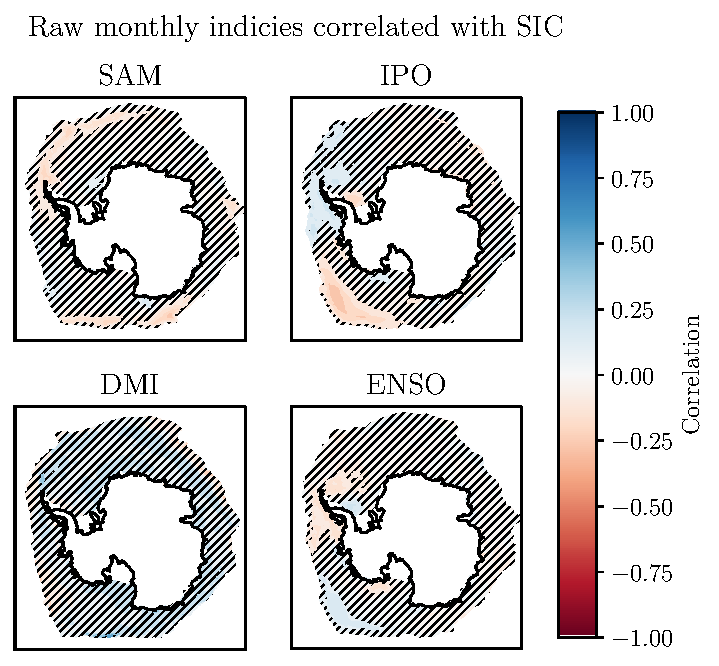
\includegraphics{images_v2/correlations/spatial/raw_monthly_raw_1_nsidc.pdf}
    \caption[Raw monthly indices correlated with SIE at individual gridpoints around Antarctica.]{Raw monthly indices correlated with SIE at individual gridpoints around Antarctica from the NSIDC dataset. Blue indicates a positive correlation and red indicates a negative correlation. Regions with a p-value larger than 0.05 has been hashed out. The unhatched regions are statistically significant.}
    \label{fig:my_label}
\end{figure}

The results above make sense but do not tell us a lot, other than highlighting that the western side of Antarctica seems to be more significantly related to the different indices. This may be due to the geography of the Antarctic peninsula.